\documentclass[lettersize,journal]{IEEEtran}
\usepackage{amsmath,amsfonts}
\usepackage{algorithmic}
\usepackage{algorithm}
\usepackage{array}
\usepackage[caption=false,font=normalsize,labelfont=sf,textfont=sf]{subfig}
\usepackage{textcomp}
\usepackage{stfloats}
\usepackage{url}
\usepackage{verbatim}
\usepackage{graphicx}
\usepackage{cite}

%\usepackage{float}
%\usepackage{multirow}
%\usepackage{tabularx}
%\usepackage{authblk}
\usepackage{booktabs}
\hyphenation{op-tical net-works semi-conduc-tor IEEE-Xplore}
% updated with editorial comments 8/9/2021

\begin{document}
\title{Defending Byzantine Attacks in Ensemble Federated Learning: A Reputation-based Phishing Approach}
\author{Beibei~Li,~\IEEEmembership{Member,~IEEE,}
        Peiran~Wang,~\IEEEmembership{Student Member,~IEEE,}
        Qinglei~Kong,~\IEEEmembership{Member,~IEEE,}
        Yuan~Zhang,~\IEEEmembership{Member,~IEEE,}
        and~Rongxing~Lu,~\IEEEmembership{Fellow,~IEEE}
\thanks{This paper is an extended version of the paper titled `FLPhish: Reputation-Based Phishing Byzantine Defense in Ensemble Federated Learning', which was published in IEEE ISCC 2021, and awarded `Best Paper'.}
\thanks{B. Li and P. Wang are with the School of Cyber Science and Engineering, Sichuan Universsity, Chengdu, Sichuan, China 610065. Email: libeibei@scu.edu.cn; wangpeiran@stu.scu.edu.cn.}
\thanks{Q. Kong is with the Future Network of Intelligence Institute, The Chinese University of Hong Kong, Shenzhen, China 518172, and also with The University of Science and Technology of China, Hefei, China 230052. Email: kql8904@163.com.}
\thanks{Y. Zhang is with the School of Computer Science and Engineering, University of Electronic Science and Technology of China, Chengdu, China 610054. Email: zy\_loye@126.com.}
\thanks{R. Lu is with the Faculty of Computer Science, University of New Brunswick, Fredericton, NB, Canada E3B 5A3. Email: rlu1@unb.ca.}
}

% The paper headers
\markboth{IEEE TRANSACTIONS ON INFORMATION FORENSICS AND SECURITY}%
{Li \MakeLowercase{\textit{et al.}}: Defending Byzantine Attacks in Ensemble Federated Learning: A Reputation-based Phishing Approach}

\IEEEpubid{0000--0000/00\$00.00~\copyright~2021 IEEE}
% Remember, if you use this you must call \IEEEpubidadjcol in the second
% column for its text to clear the IEEEpubid mark.

\maketitle

\begin{abstract}
  Emerging as a promising distributed learning paradigm, federated learning (FL) has been widely adopted in many fields. Nonetheless, a big challenge for FL in real-world implementation is Byzantine attacks, where compromised clients can mislead or poison the training model by falsifying or manipulating the local model parameters. To solve this problem, in this paper, we present a reputation-based Byzantine robust-FL scheme (called FLPhish) for defending Byzantine attacks under the Ensemble Federated Learning architecture (called EFL). Specifically, we first develop a novel ensemble FL architecture, EFL, which allows FL compatible with different deep learning models in different clients. Second, we craft a phishing algorithm for the EFL architecture to identify possible Byzantine behaviors. Third, a Bayesian inference based reputation mechanism is devised to measure each client's level of confidence and to further identify Byzantine clients. Last, we strictly analyze how the FLPhish scheme defend against backdoor attacks. Extensive experiments under different settings demonstrate that the proposed FLPhish achieves great efficacy in defending Byzantine attacks in EFL. FLPhish is tested with different fractions of Byzantine clients and different degrees of distribution imbalance. \cite{ref_01_GoogleFL}
\end{abstract}

\begin{IEEEkeywords}
  Federated learning, ensemble learning, Bayesian inference-based reputation, phishing.
\end{IEEEkeywords}

\begin{table}[t]
  \caption{Summary of Notations}
  \resizebox{0.5\textwidth}{!}{
  \begin{tabular}{lp{6cm}}
    \bottomrule
    Term&Description\\
    \hline
    $s$ & central server in FL \\
    $c_i$ & the $i$th client in FL, $i=1,2,3,...,u$ \\
    $d_i$ & the local dataset preserved by the $i$th client \\
    $C$ & the ensemble of all the clients \\
    $u$ & the number of clients\\
    $D_t$ & the unlabeled dataset chosen by $s$ in each procedure\\
    $D$ & the unlabeled dataset preserved by $s$\\
    $n$ & the number of samples in $D_t$\\
    $B_t$ & the labeled dataset (\textit{`bait'}) chosen by $s$ in each procedure\\
    $B$ & the labeled dataset preserved by $s$\\
    $m$ & the number of samples in $B_t$\\
    $a_i^t$ & the accuracy of predictions of $B_t$ made by $c_i$ in $t$th procedure\\
    $q_i$ & the label of $c_i$ to judge it is a malicious client or not\\
    $r_q$ & the threhold of malicious clients\\
    $x^t_l$ & the $l$th data point in $D_t$\\
    $b_i$ & the Byzantine attacker\\
    $\sigma$ & the `trigger' in the backdoor attack\\
    $\iota$ & the backdoor label in the backdoor attack\\
    $\mathbf{M}$ & global model preserved by $s$\\
    $\mathbf{m_i}$ & local models trained by the $i$th client\\
    $\mathbf{k_i^t}$ & the predictions (\textit{`knowledge'}) made by the $i$th client in the $t$th procedure\\
    $\mathbf{\hat{y}^t_l}$ & the ensembled prediction of data point $x^t_l$\\
    $\mathbf{\hat{y}^i_l}$ & the prediction of $l$th data point made by $i$th client\\
    $\mathbf{K_t}$ & the aggregated labels (predictions) of the $t$th iteration's unlabeled dataset\\
    \hline
  \end{tabular}
  }
\end{table}



\section{Conclusion}
The conclusion goes here.


\section*{Acknowledgments}
This should be a simple paragraph before the References to thank those individuals and institutions who have supported your work on this article.



{\appendix[Proof of the Zonklar Equations]
Use $\backslash${\tt{appendix}} if you have a single appendix:
Do not use $\backslash${\tt{section}} anymore after $\backslash${\tt{appendix}}, only $\backslash${\tt{section*}}.
If you have multiple appendixes use $\backslash${\tt{appendices}} then use $\backslash${\tt{section}} to start each appendix.
You must declare a $\backslash${\tt{section}} before using any $\backslash${\tt{subsection}} or using $\backslash${\tt{label}} ($\backslash${\tt{appendices}} by itself
 starts a section numbered zero.)}



%{\appendices
%\section*{Proof of the First Zonklar Equation}
%Appendix one text goes here.
% You can choose not to have a title for an appendix if you want by leaving the argument blank
%\section*{Proof of the Second Zonklar Equation}
%Appendix two text goes here.}



\section{References Section}
You can use a bibliography generated by BibTeX as a .bbl file.
 BibTeX documentation can be easily obtained at:
 http://mirror.ctan.org/biblio/bibtex/contrib/doc/
 The IEEEtran BibTeX style support page is:
 http://www.michaelshell.org/tex/ieeetran/bibtex/
 
 % argument is your BibTeX string definitions and bibliography database(s)
%\bibliography{IEEEabrv,../bib/paper}
%
\section{Simple References}
You can manually copy in the resultant .bbl file and set second argument of $\backslash${\tt{begin}} to the number of references
 (used to reserve space for the reference number labels box).


 \bibliography{IEEEabbrv}
\begin{thebibliography}{1}
\bibliographystyle{IEEEtran}

\bibitem{ref1}
{\it{Mathematics Into Type}}. American Mathematical Society. [Online]. Available: https://www.ams.org/arc/styleguide/mit-2.pdf

\bibitem{ref2}
T. W. Chaundy, P. R. Barrett and C. Batey, {\it{The Printing of Mathematics}}. London, U.K., Oxford Univ. Press, 1954.

\bibitem{ref3}
F. Mittelbach and M. Goossens, {\it{The \LaTeX Companion}}, 2nd ed. Boston, MA, USA: Pearson, 2004.

\bibitem{ref4}
G. Gr\"atzer, {\it{More Math Into LaTeX}}, New York, NY, USA: Springer, 2007.

\bibitem{ref5}M. Letourneau and J. W. Sharp, {\it{AMS-StyleGuide-online.pdf,}} American Mathematical Society, Providence, RI, USA, [Online]. Available: http://www.ams.org/arc/styleguide/index.html

\bibitem{ref6}
H. Sira-Ramirez, ``On the sliding mode control of nonlinear systems,'' \textit{Syst. Control Lett.}, vol. 19, pp. 303--312, 1992.

\bibitem{ref7}
A. Levant, ``Exact differentiation of signals with unbounded higher derivatives,''  in \textit{Proc. 45th IEEE Conf. Decis.
Control}, San Diego, CA, USA, 2006, pp. 5585--5590. DOI: 10.1109/CDC.2006.377165.

\bibitem{ref8}
M. Fliess, C. Join, and H. Sira-Ramirez, ``Non-linear estimation is easy,'' \textit{Int. J. Model., Ident. Control}, vol. 4, no. 1, pp. 12--27, 2008.

\bibitem{ref9}
R. Ortega, A. Astolfi, G. Bastin, and H. Rodriguez, ``Stabilization of food-chain systems using a port-controlled Hamiltonian description,'' in \textit{Proc. Amer. Control Conf.}, Chicago, IL, USA,
2000, pp. 2245--2249.

\end{thebibliography}


\newpage

\section{Biography Section}
If you have an EPS/PDF photo (graphicx package needed), extra braces are
 needed around the contents of the optional argument to biography to prevent
 the LaTeX parser from getting confused when it sees the complicated
 $\backslash${\tt{includegraphics}} command within an optional argument. (You can create
 your own custom macro containing the $\backslash${\tt{includegraphics}} command to make things
 simpler here.)
 
\vspace{11pt}

\bf{If you include a photo:}\vspace{-33pt}
\begin{IEEEbiography}[{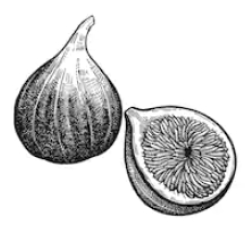
\includegraphics[width=1in,height=1.25in,clip,keepaspectratio]{fig1}}]{Michael Shell}
Use $\backslash${\tt{begin\{IEEEbiography\}}} and then for the 1st argument use $\backslash${\tt{includegraphics}} to declare and link the author photo.
Use the author name as the 3rd argument followed by the biography text.
\end{IEEEbiography}

\vspace{11pt}

\bf{If you will not include a photo:}\vspace{-33pt}
\begin{IEEEbiographynophoto}{John Doe}
Use $\backslash${\tt{begin\{IEEEbiographynophoto\}}} and the author name as the argument followed by the biography text.
\end{IEEEbiographynophoto}




\vfill

\end{document}


